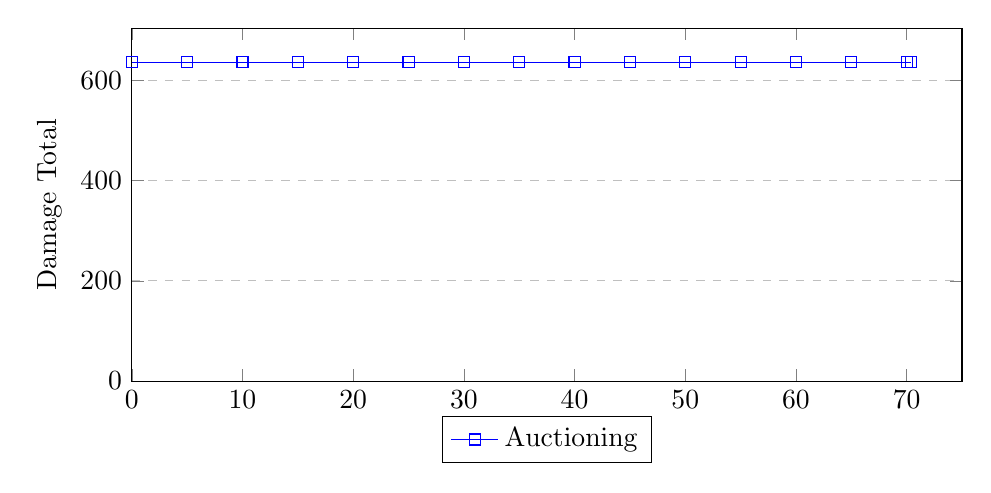
\begin{tikzpicture}
\begin{axis}[
    xlabel={Timestamp [s]},
    ylabel={Damage Total},
    xmin=0, xmax=75000,
    ymin=0, ymax=704,
    legend columns=-1,
    legend style={at={(0.5,-0.1)},anchor=north},
    ymajorgrids=true,
    grid style=dashed,
    width=\textwidth,
    height=0.5\textwidth,
    scaled x ticks=base 10:-3,
    xtick scale label code/.code={}
]

	\addplot[color=blue,mark=square] coordinates {
        (0,636.01)(5000,636.01)(10000,636.01)(15000,636.01)(20000,636.01)(25000,636.01)(30000,636.01)(35000,636.01)(40000,636.01)(45000,636.01)(50000,636.01)(55000,636.01)(60000,636.01)(65000,636.01)(70000,636.01)(70357,636.01)
    };
    \addlegendentry{Auctioning}




\end{axis}
\end{tikzpicture}